\chapter{Identity and Trajectory Construction}

%123456789 123456789 123456789 123456789 123456789 123456789 123456789 123456789

In this chapter we focus on actual techniques how to group detections into
desired clusters, i.e. creating \glspl{iden} as per \autoref{ssec:task}.
We show how we combine visual information of the image
(\autoref{ch:features}) with metadata to provide \glspl{iden}.

\section{Trajectories}

In this section, we focus on grouping \glspl{det} together by the object they
capture without the visual information, i.e. purely based on the metadata. In
other words we create trajectories as per \autoref{sec:workflow}. By its nature
the \glspl{det} within single trajectory are from consecutive frames and
physically close together.

The reason for this step is to group the \glspl{det} together in cases
where the visual information --- which processing may be complicated --- is not
needed. They then further serve as a ``building blocks'' for subsequent
processes.


% The trajectories serve as a ``building blocks'' for more
% complicated \glspl{iden}. Due to the way they are constructed the trajectories
% are clusters of \glspl{det} that are physically close together. They are usually
% just list of \glspl{det} from the consecutive frames with just a minor changes
% in position of tracked object in-between the frames.

\subsection{Detection Metadata}

Let us briefly recall available metadata for each \gls{det} as introduced in
\autoref{ssec:input}:

\begin{itemize}
    \item $(x_0, x_1, y_0, y_1)$ -- Position of the bounding box of the detection given by $x$-coordinate of the left and the right edge and the $y$-coordinate of top and bottom edge respectively.
    \item $v$ -- Class of the detection, e.g. person, car or truck
    \item $c$ -- Identificator of a the camera
    \item $t$ -- Timestamp
\end{itemize}


Let us start with a simplification. We consider metadata of just two
\glspl{det} at hand, and we explore if we can find out whether the \glspl{det}
display the same object. We discuss this \gls{iden} correspondence for each part
of the metadata separately.

\subsection{Processing of simple metadata information}

Let us start with the metadata regarding the class of the object. The class
gives us the most straight-forward conclusion.
If the two \glspl{det} at hand are of different classes we know for sure
that they can not be of the same \gls{iden} (i.e. displaying the same
object).\footnote{There is quite
odd case where this seemingly obvious conclusion can be argued against. That
is, for example, when a person enters a car. Based on the actual definition of
the \gls{iden} we may consider it the same displayed object. As these cases
raises multiple questions (e.g. what should happen when multiple people enters the same vehicle), we shall
consider person entering the vehicle and the vehicle itself as different
\glspl{iden} and we leave further research in this topic to
future work.} As a corollary, we therefore assume that the two \glspl{det} are
of the same class while investigating the rest of the metadata (as in the
opposite case we reject that they are of same object).

We can incorporate identificator of the camera just as easily. If the two
\glspl{det} are from different cameras, we do not explore the remaining
metadata, as they do not hold any useful information in such
case.\footnote{There
are approaches that assume that the two given cameras capture largely the same
camera and are calibrated (for example \cite{hu2006principal}). However, we
assume no prior calibration and therefore we leave similar approaches to other
work} For example even if there is one detection in top left corner of one
camera, and in exact same time there is another detection in top left corner
of another camera at the same time, we can not say if the \glspl{det}
display the same person or not. This is
because we do not know if the area within top left corner is the same as the
area in the top left corner of the second camera. In such case we have to use
a priori assumption and assign them to two different
trajectories.\footnote{Unless we have any additional information the a priori
assumption that two detections belong to the same golnden \gls{iden} is more
likely to be true than the opposite if there is no
golden trajectory that would be represented by more than a half of the
\glspl{det} within given \gls{ses}, which seems like a reasonable assumption to
have}

For assignment into the same trajectory we therefore consider only \glspl{det}
from the same camera. Therefore we only elaborate on such cases in the remainder
of this subsection. We regard cases how to discover the same object across
different cameras later in this chapter (\autoref{sec:generating_identities}).

% Nevertheless, it still may be true that the \glspl{det} display the same
% object and we may discover it by processes described later in this chapter.
% However, for the purpose of generating trajectories we process the information
% about camera as described and for the remainder of this section we assume the
% case where the \glspl{det} are from the same camera.

Lastly, us consider additional information that we gain by using the timestamp.
With combination with the spatial data the timestamp can be helpful. However as
we mentioned in the intro of this section
we are now interested in creating short trajectories (i.e. clusters of
\glspl{det} that are physically close together). Therefore
our approach to temporal information is be simple: If the time difference is
bigger than selected threshold (say 1 second, however we experiment with
various settings), we assign the \glspl{det} to different trajectories. In the
opposite case we shall further evaluate secondary conditions on the spatial
information.

\subsection{Conditioning on spatial information}

\label{ssec:spatial_merging}

Let us derive a couple of quantities that may be useful for us when deciding
if we should assign given \glspl{det} to same trajectory. Deciding if we should
assign them to the same trajectory is then just a matter of comparing one or
more of the following quantities with pre-selected threshold. If we find pair
of detection where all the considered quantities are less than corresponding
threshold, we shall merge the trajectories together.

For brevity in the following lines we shall use height ($h = y_1 - y_0$) and
width ($w = x_1 - x_0$) of a detection.

\subsubsection{Displacement}

One of the obvious quantities to consider when comparing two \glspl{det} is
their displacement. We shall compute the displacement with respect to centers
of the \glspl{det}. Formally we can compute a displacement as follows
(superscripts represent which \gls{det} the values are from)

\begin{align*}
    c^{(A)} &= \left(\frac{x_0^{(A)} + x_1^{(A)}}{2}, \frac{y_0^{(A)} + y_1^{(A)}}{2}\right) \\
    c^{(B)} &= \left(\frac{x_0^{(B)} + x_1^{(B)}}{2}, \frac{y_0^{(B)} + y_1^{(B)}}{2}\right) \\
    d &= \delta_{euclid}(c^{(A)}, c^{(B)})
\end{align*}

\subsubsection{Relative Displacement}

However, such simple displacement only express the displacement within the
screen of the camera. If an object close to the camera moves, this movement
will translate to large movement within the screen of the camrea, but if we
perceive the same movement by an object further from the camera, the percieved
movement will be much greater. Luckily, we can estimate the ``closeness'' to the
camera without the prior calibration. Simply by considering the size of the
bounding box of the detection (i.e. bigger the bounding box, more likely it is
that the object is closer to the camera). This works especially if the project
are usually of the same size (i.e. all people). While this estimation is qutie
vague, it has other advantages. For example it also ``expects'' smaller objects
(i.e. kids) to make smaller movements than bigger ones. Nevertheless, this leads
us to the definition of relative displacement where we divide the displacements
by average edge length of the bounding boxes:

$$\frac{d}{\left(h^{(A)} + w^{(A)} + h^{(B)} + w^{(B)}\right) / 4}$$

\subsubsection{Intersection over Union}

The last quantity we shall consider when merging \glspl{det} to trajectories is 
so-called intersection over union. It is simply area covered by both boundign
boxes (i.e. union) divided by area covered by both bounding boxes (i.e.
intersection). For visual interpretation see \autoref{fig:iou}. Formally we can
define the quantity for our rectangular bounding boxes as:

\begin{align*}
    \text{InterWidth} &= \min\left(x_1^{(A)}, x_1^{(B)}\right) - \max\left(x_0^{(A)}, x_0^{(B)}\right) \\
    \text{InterHeight} &= \min\left(y_1^{(A)}, y_1^{(B)}\right) - \max\left(y_0^{(A)}, y_0^{(B)}\right) \\
    \text{Intersection} &= \begin{cases}\text{InterWidth} \cdot \text{InterHeight} & \text{if InterWidth} > 0 \land \text{InterHeight} > 0 \\ 0 & \text{else}\end{cases} \\
    \text{Union} &= w^{(A)} h^{(A)} + w^{(B)} h^{(B)} - \text{Inter} \\
    \text{IoU} &= \frac{\text{Intersection}}{\text{Union}}
\end{align*}

\begin{figure}
    \centering
    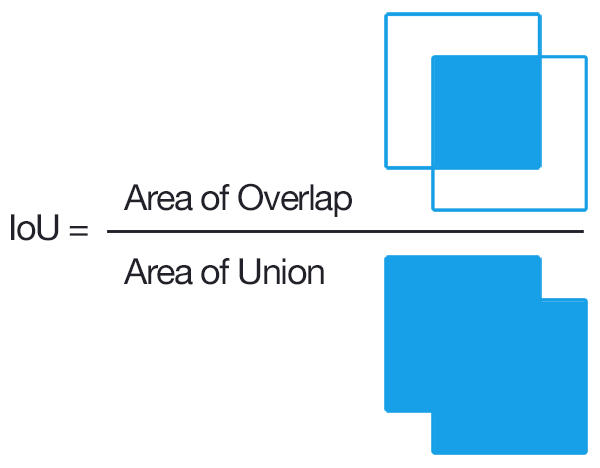
\includegraphics[width=6cm]{img/Intersection_over_Union_-_visual_equation.png}
    \caption[Visualization of intersection over union]{Visualization of intersection over union\\Source: Intersection over Union -- visual equation\footnote{\url{https://commons.wikimedia.org/wiki/File:Intersection_over_Union_-_visual_equation.png}} by Adrian Rosebrock, CC BY-SA 4.0\footnote{\url{https://creativecommons.org/licenses/by-sa/4.0}}, via Wikimedia Commons}
    \label{fig:iou}
\end{figure}

\subsection{Trajectory generation}

\label{ssec:trajectory_generation}

In this section we show how we generate local trajectories based on
the information overviewed in previous section. Comparing every \gls{det} with
every other \gls{det} takes quadratic time with respect to number of detection
and for hundredths of thousands of \glspl{det} is unfeasible to compute on
standard hardware. Therefore, we need to lower the number of comparison.

We leverage the way we incorporated timestamp into trajectory generation
we described in previous subsection. By considering only
\glspl{det} under given threshold allows us to compare only \glspl{det} by using
sliding window. We shall process the \glspl{det} in order of their timestamp.
When we process a new \gls{det} we add it to the sliding window. At the same
time we remove all the \glspl{det} from the window that are older than the
timestamp of the new detection minus the threshold. Then we compare the new
\gls{det} with all the \glspl{det} within the window. This dramatically decrease
the number of comparison compared to approach where we compare all the
\glspl{det} with every other \gls{det}.

However, this approach does not mean that the length of the trajectories is
bounded by the given time threshold. We use ``transitive'' information about
the trajectory. Namely, we know it a \gls{det} (A) belongs to the same
trajectory as \gls{det} (B) and \gls{det} (B) belongs to same trajectory as 
\gls{det} (C), we can conclude that the \gls{det} (A) and \gls{det} (C) is of
same trajectory. We shall use standard union-find (originally described by
\cite{galler1964improved}) architecture which allows us to track which \glspl{det} belongs to which trajectory and merge them in almost
constant\footnote{The actual complexity of the operation is inverse
Ackermann function of the size of the structure per query (amortized) as were
proved by \cite{tarjan1984worst}. For the details of the structure please refer
to the attached code or the original research.} time per request.
Furthermore, such approach allows us
to set the threshold to stricter values and still capture via ``transitive''
property the full length of the trajectory.

\section{Identities}

\label{sec:generating_identities}

So far we have looked into how to construct trajectories.
There are just a few steps to merge these trajectories together to fulfill
our original goal. That is to obtain clusters of detection where each cluster
contains all the detection display the same object -- i.e. what we define
as \gls{iden}.
\todo{Preformulovat}

\subsection{Trajectory merging}

We merge the trajectories to bigger \glspl{iden} by incorporating the visual
information. The rationale is that we used all metadata which allowed us to
cluster \glspl{det} that were physicially close together to trajectories.
Now we make use of the visual information we have in form of the feature vectors
(generated by approaches described in \ref{ch:features}) to connect \glspl{det}
that may be physically distant or recorded on different cameras to obtain
\glspl{iden}.

The key information in this step is the distance between the feature
vectors of \glspl{det}. We shall explore multiple distance functions
(Euclidean, Manhattan, Cosine -- for definitions please refer to
\autoref{sec:distances}) and their effect on the quality of resulting
\glspl{iden}.

The straight-forward approach is to use the same algorithm as when we
generated the trajectories, except that use the feature vectors
rather than metadata. In this approach we decide if we marge two trajectories
together by comparing feature vectors of their \glspl{det} and their distance
with respect to selected distance function. If for any pair of \glspl{det} 
(one \gls{det} from each trajctory) the computed distance is lower then selected
threshold, we merge the trajectories together. This requires to compute distance
between each \gls{det} from the first trajectory with each \gls{det} of the
second trajectory. Hence this again leads to quadratic complexity.
Therefore, we present a way to decrease this number significantly.

\subsubsection{Representant Selection}

We present a relatively simple approach to decrease number of comparison needed.
The idea behind the approach is to select from each trajectory a set of
representants. We want to select a  suitable set of representsnts that will
preserve all information needed for creating appropriate \glspl{iden}.

To pick the representant effectively we make a simple observation. Let there be
two different \glspl{det} within a trajectory, that are fairly similar. Then
whenever we want to decide if we want to add another \gls{det} into a trajectory
we need to compare the \gls{det} to just one of the original \gls{det}. The
point is that while the measured distance may be grater than when compared
to the other of two \glspl{det}, due to the triangular inequality, the distance
will be greater at most by the distance between two original \glspl{det}.
As noted this observation depends on triangle inequality and thus holds only
for metric functions.
For systematic way of how to select representnts using this observation
see \autoref{alg:representants}.

We can apply this observation in a context of more than just three \glspl{det}.
Let us assume that we  start with trajectories that are ``clean'' (i.e.
trajectory contain \glspl{det} of just a single golden \gls{iden}). Further
assume that the golden \glspl{iden} are ``well-separated'' using the selected
metric function in a following sense: The minimal distance between two
\glspl{det} from different golden \glspl{iden} is at least $\Delta_{mrg}$
and for every pair of \glspl{det} from any \gls{iden} there exists a sequence
of \glspl{det} such that every \gls{det} is from the same \gls{iden} and
and distance between two consecutive \glspl{det} is at most
$\Delta_{mrg} - 2\Delta_{rep}$. Then the produced \glspl{iden} produced by
selection representants by \autoref{alg:representants} and then merging
trajectories that have \glspl{det} closer than $\Delta_{mrg}$
are always exactly golden \glspl{iden}.


% The observation that will help us select proper representative is that if
% there are two \glspl{det} within a trajectory, that are similar (in terms of
% distance between their feature vectors), than whatever third \gls{det} is
% similar to the first \gls{det} is similar also to second \gls{det} (at least
% as long as we use metric and not generic distance as we show in a while).
% Therefore if there is a pair of similar \glspl{det} in a trajectory, we select
% at most one as a representant and discard the other. For systematic way of
% selecting representant leveraging this property see \autoref{alg:representants}.


\begin{algorithm}
 \SetKwInOut{Input}{input}
 \SetKwInOut{Output}{output}

 \Input{Trajectory $T$ (as a list of feature vectors of detections), Threshold $t$}
 \Output{List of feature vectors of representants}
 
 \BlankLine
 $R \leftarrow$ \emph{empty list}\;
 \For(\tcp*[h]{outer loop}){$D_{new} \in T$}{
  \For{$D_{rep} \in R$}{
   \If{$\delta(D_{new}, D_{rep}) \leq t$}{
    skip on next iteration of outer loop\;
   }
  }
  append $D_{new}$ to $R$\;
 }
 \Return $R$
 \caption{Selection of representants of a trajectory}
 \label{alg:representants}
\end{algorithm}

% Our intuitive observation, that we need to preserve only one of the two similar
% \glspl{det} in a trajectory can be formalized as:

This claim can be formalized as follows:

\begin{figure}
    \centering
    \def\svgwidth{\columnwidth}
    \input{img/claim.pdf_tex}
    \caption[Visualization of \autoref{clm:claim}]{Visualization of  \autoref{clm:claim}. The figure shows two \glspl{iden}, first of them dividen into three trajectories, latter into two. White dots represents \glspl{det}, black dots represent \glspl{det} which were chosen as representants. Solid lines (shown only is the first trajectory) shows shortest distance to a representant, such distances are are most $\Delta_{rep}$. Dashed lines shows distances between representants, such distances are greater than $\Delta_{rep}$. Dotted lines shows some distances between \glspl{det} of different trajectories of the same \gls{det}. The claim considers situations where all such distances are at most $\Delta_{mrg} - 2\Delta_{rep}$. If such distance between two representants are at most $\Delta_{mrg}$, the corresponding trajectories will be merged together (i.e. they are in $\circ$ relation. The grey lines are distances between \glspl{det} of different \glspl{iden}, the claim considers cases where such distances are greater than $\Delta_{mrg}$}
    \label{fig:claim}
\end{figure}

\begin{claim}
\label{clm:claim}
Let:

\setlength{\itemsep}{0pt}
\setlength{\parskip}{0pt}

\begin{itemize}
    \item $D$ be a set of \glspl{det}
    \item $A$ a partitioning of $D$ (this represents golden \glspl{iden})
    \item $T$ partitioning of $D$ such that $(\forall t \in T) (\exists a \in A) (t \subseteq a)$ (this represents input ``clean'' trajectories)
    \item $\Delta_{rep}, \Delta_{mrg} \in \R^+$ such that $\Delta_{rep} < \Delta_{mrg}$
    \item $\delta$ be an metric function over $D$
    \item $r$ be a function $r: \Pt{D} \goto \Pt{D}$ such that $(\forall c \subseteq D) (\forall b \in c) (\exists b' \in r(c)) (\delta(b, b') \leq x_{rep})))$ (this represents selection of representants obtained for example via \autoref{alg:representants})
    \item $\circ$ be a relation over $T$ such that $t\circ t' \Leftrightarrow (\exists d \in r(t)) (\exists d' \in r(t')) (\delta(d, d') \leq x_{mrg})$ (two trajectories are in relation $\circ$ if we can merge them together)
    \item $\bullet$ be a transitive closure of $\circ$ (i.e. $t \bullet t' \Leftrightarrow (\exists n \in \N) (\exists (t_1, \ldots, t_n) \in T^n) (t = t_1 \land t' = t_n \land (\forall i) (t_i\circ t_{i+1}))$ (this relation is equivalence that represents final \glspl{iden} -- two trajectories are in relation $\bullet$ if and only if they were merged together)
\end{itemize}

If the following holds (i.e. the golden \glspl{iden} are ``well-separated''):
\begin{itemize}
    \item $(\forall a \in A)(\forall d, d' \in a) (\exists n \in \N) (\exists (d_1, \ldots, d_n) \in D^n) (d = d_1 \land d' = d_n \land (\forall i) (\delta(d_i, d_{i+1}) \leq x_{mrg} - 2x_{rep}))$
    \item $(\forall a, a' \in A) (\forall d \in a) (\forall d' \in a') (a \neq a' \Rightarrow \delta(d, d') > x_{mrg})$
\end{itemize}

Then: $t\bullet t' \Leftrightarrow (\exists a \in A) (t \cup t' \subseteq a)$ (i.e. produced \glspl{iden} exactly match golden \glspl{iden})

% Let $D$ be a set of \glspl{det}, $A$ its partitioning, $\delta$ a metric over
% $D$, $T$ another partitioning of $D$ such that $(\forall t \in T) (\exists a \in A) (t \subseteq a)$ and thresholds $x_{rep}, x_{merge} \in \R^+$. Denote $r: \Pt{D} \goto \Pt{D}$ generator representants as per \autoref{alg:representants} with threshold $x_{rep}$. Now consider $R$ to be a relation over $T$ such that $tRt' \Leftrightarrow (\exists d \in r(t)) (\exists d' \in r(t')) (\delta(d, d') \leq x_{merge})$ and let $\widehat{R}$ be its transitive closure.

% If $\min_{a, a' \in A : a \neq a'} \min_{d \in a, d' \in a'} \delta(d, d') > x_{merge}$ and
% $(\forall a \in A)(\forall d, d' \in a)(\exists (d = d_1, d_2, \ldots, d_n = d') \subseteq a)(\forall i)(\delta(d_i, d_{i+1}) \leq x_{merge} - 2x_{rep})$ 
% then $t\widehat{R}t' \Leftrightarrow (\exists a \in A)(t \cup t' \subseteq a)$.

\end{claim}

% This claim basically tells us that if we start with the trajectories that
% are ``clean'' (i.e. each trajectory is a subset of some golden \gls{iden}) and
% the \glspl{iden} are well-separated (i.e. distance between golden \glspl{iden}
% are at least $x_{merge}$ and for any pair of the \glspl{det} within a \gls{iden}
% there is a sequence of \glspl{det} such thateach subseqent pair of \glspl{det} within the sequence is distant at most $(x_{merge} - 2x_{rep})$ and the ends
% of the sequence are the original two \glspl{det}, then the produced clustering
% of the \glspl{det} corresponds to the desired golden \glspl{iden}.

\begin{myproof}
First, let us prove that $t \bullet t' \Rightarrow (\exists a \in A) (t \cup t' \subseteq a)$. We shall prove this by contradiction, i.e. for now we assume
that $(\exists a \in A) (t \in a)$ and $(\exists a' \in A) (t' \in a')$ and $a \neq a'$. From property of $\bullet$ we know there is a sequence of $t_1, t_2, \ldots t_n$ (for some $n$), such that $(\forall i) (t_i \circ t_{i+1})$. Let
us take minimal $i$ such that $t_i$ and $t_{i+1}$ is not subset of the same
$a \in A$ (such $i$ exists as $t$ and $t'$ does belong to different $a$s).
For such $i$ (since $t_i \circ t_{i+1}$) there is $d \in t_i$ and
$d' \in t_{i+1}$ such that $\delta(d, d') \leq x_{mrg}$. However since $d \in a$
and $d' \in a'$ (such that $a \neq a'$) this is in contradiction with second
of the original assumptions.

Now let us prove that $(\exists a \in A) (t \cup t' \subseteq a) \Rightarrow t \bullet t'$. Let us choose $d \in t$ and $d' \in t'$ arbitrarily. By the
assumptions for elements of $a$ there is sequence $(d_0, \ldots, d_n) \in A^n$
such that $d = d_0 \land d' = d_n \land (\forall i) (\delta(d_i, d_{i+1}) \leq x_{mrg} - 2x_{rep}$. Now let us denote for each $i$ $t_i \in T$ such that
$d_i \in t_i$. Finally, let us denote $r_i = \mathrm{argmin}_{d \in r(t_i)} \delta(d, d_i)$. If $t_i = t_{i+1}$ then $t_i \circ t_{i+1}$ by definition.
So let us consider cases where $t_i \neq t_{i+1}$. In such case we can bound
the distance between $r_i$ and $r_{i+1}$ due to the triangle inequality:
$\delta(r_i, r_{i+1}) \leq \delta(r_i, d_i) + \delta(d_i, d_{i+1}) + \delta(d_{i+1}, r_{i+1}) \leq x_{rep} + (x_{mrg} - 2x_{rep}) + x_{rep} = x_{mrg}$. And as $r_i \in r(t_i)$ we can conclude that $(\forall i) (t_i \circ t_{i+1})$. Therefore $t \bullet t'$.\end{myproof}


\begin{cor}
If the distance between two closest \glspl{det} from different golden
\glspl{iden} is $\Delta_{between}$ and the distance between two most distance detection
of the same golden \gls{iden} is $\Delta_{within} < \Delta_{between}$, then for any set of ``clean''
trajectories (i.e. if each trajectory contains \glspl{det} only from single
golden \gls{iden}) the \autoref{alg:representants} for representant selection
with threshold $(\Delta_{between} - \Delta_{within} - \varepsilon) / 2$ (for arbitrarily small
$\varepsilon \in \R^+$) followed by merging based on representants with
threshold $\Delta_{between} - \varepsilon$ produces the golden \glspl{iden}.
\end{cor}

Let us note that the original assumption is fulfilled if the Triplet Loss
over the examinated dataset is zero (and in some cases even if it is positive).
This is usually too strong assumption to make, however it still gives us some
theoretical justification for our approach.

In case that $\delta$ is not metric function but just a generic distance
function we have no such guarantees. However we still evaluate this approach
even for such distance functions.

\subsection{Direct identity generation}

So far we have presented two-step approach. In the first step we generate
trajectories and during the second step we merge these trajectories into
final \glspl{iden}.

However, we also experiment with the approach where we
generate the identities directly. This approach would work similar as to
original trajectory detection where we have a sliding window of \glspl{det}
and we merge two sets of \glspl{det} together if we find two similar
\glspl{det}. This approach has significant drawback of not being able to
merge two sets of \glspl{det} together if there is too big ``time gap'' between
two consecutive \glspl{det}. Nevertheless, we believe it is worth to experiment
with this direct approach.

However, we still want to be able to at least assign two \glspl{det} to the
same \gls{iden} if they both fit into the sliding window, even though they are
from different cameras. Therefore, our approach will be as follows: If we are
considering two \glspl{det} for merging, we evaluate the spatial information
exactly as in \autoref{ssec:spatial_merging}. If all the conditions are met,
then we merge corresponding set of \glspl{det}. If one of the threshold is
exceeded then we evaluate the visual information. If the corresponding feature
vectors are closer then pre-selected threshold then we do the merge even though
the information from metadata is not conclusive.

\section{Recapitulation}

In this chapter we elaborated on two ways of generating \glspl{iden} that we
experiment with (trajectory generation with subsequent merging and direct
approach). Both are dependent on which feature vectors will be used (which we
described in \autoref{ch:features}). Furthermore, each approach is dependent
on selection of various thresholds, we experiment with various setting of those
thresholds. The list of quantities with threshold is:

\begin{itemize}
    \item Size of the sliding window
    \item Displacement
    \item Relative displacement
    \item Intersection over Union
    \item Visual distance
\end{itemize}